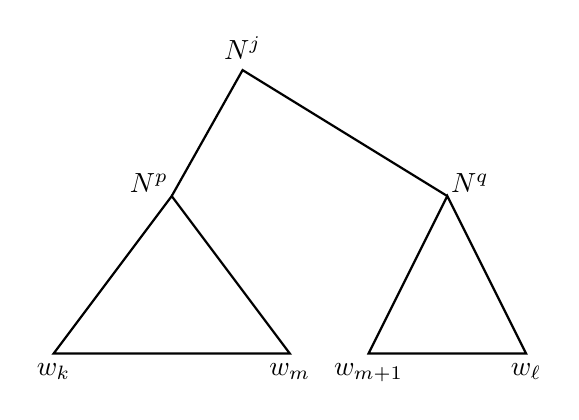
\begin{tikzpicture}[thick]
  \coordinate (Nj) at (2.4,3.6);
  \coordinate (Np) at (1.5,2.0);
  \coordinate (Nq) at (5.0,2.0);
  \draw (Np) -- (Nj) -- (Nq);
  \draw (Np) -- (0,0) -- (3,0) -- cycle;
  \draw (Nq) -- (4.0,0) -- (6.0,0) -- cycle;
  \node[above] at (Nj) {$N^j$};
  \node[above left, inner sep=1pt] at (Np) {$N^p$};
  \node[above right, inner sep=1pt] at (Nq) {$N^q$};
  \node[below] at (0,0) {$w_k$};
  \node[below] at (3,0) {$w_m$};
  \node[below] at (4.0,0) {$w_{m+1}$};
  \node[below] at (6.0,0) {$w_\ell$};
\end{tikzpicture}
